\documentclass{beamer}
\usepackage[russian]{babel}
\usetheme{metropolis}

\usepackage{amsthm}
\usepackage{ulem}
\setbeamertemplate{theorems}[numbered]

\setbeamercolor{block title}{use=structure,fg=white,bg=gray!75!black}
\setbeamercolor{block body}{use=structure,fg=black,bg=gray!20!white}

\usepackage[T2A]{fontenc}
\usepackage[utf8]{inputenc}

\usepackage{hyphenat}
\usepackage{amsmath}
\usepackage{graphicx}

\AtBeginEnvironment{proof}{\renewcommand{\qedsymbol}{}}{}{}

\title{
Микроэкономика-I
}
\author{
Павел Андреянов, PhD
}

\begin{document}

\maketitle

\begin{frame}{План лекции}
\begin{itemize}
  \item Часть 1. Трейд + дорешать с прошлой лекции
  \item Часть 2. Больше КПВ. Повтор равновесия с производством.
\end{itemize}

Внимание, в это время, в прошлом году, я перестал регулярно перекладывать лекции в учебник, так что ориентируйтесь больше на слайды.
\end{frame}

\section{Парето всё (с консы)}
\begin{frame}{Парето всё}
На консультации я говорил о том, что максимизация взвешенной полезности это, вообще говоря, только достаточные условия, но не необходимые. Только когда все выпукло, непрерывно и строго монотонно вы получаете гарантированно (оба) Парето Фронта.
\begin{figure}[hbt]
\centering

\includegraphics[width=1 \textwidth]{pic1.png}
\end{figure}
Более того, если быть неаккуратным со знаком, то можно получить что-то вовсе неверное (см. последний пример на консультации с точками касания).
\end{frame}

\section{Трейд, пример 2 (с прошлой лекции)}

\begin{frame}{Пример 2}

Вернемся к примеру с прошлой лекции

Одна из двух стран (страна B) обладает абсолютным преимуществом в производстве всех товаров.
$$ F^A(X,Y) = X + Y/2 - 1 \leqslant 0, \quad F^B(X,Y) = X/4 + Y/2 - 1 \leqslant 0$$
Полезность Кобб Дуглас у обоих: $$U^i(x,y) = \log x + \log y, \quad i= {A,B}.$$
Напомню, что \alert{в трейде, у меня вектора $X, Y$ уже как бы содержат в себе начальные запасы.}
\end{frame}

\begin{frame}{Пример 2}
$$ F^A(X,Y) = X + Y/2 - 1 \leqslant 0, \quad F^B(X,Y) = X/4 + Y/2 - 1 \leqslant 0$$
\begin{figure}[hbt]
\centering
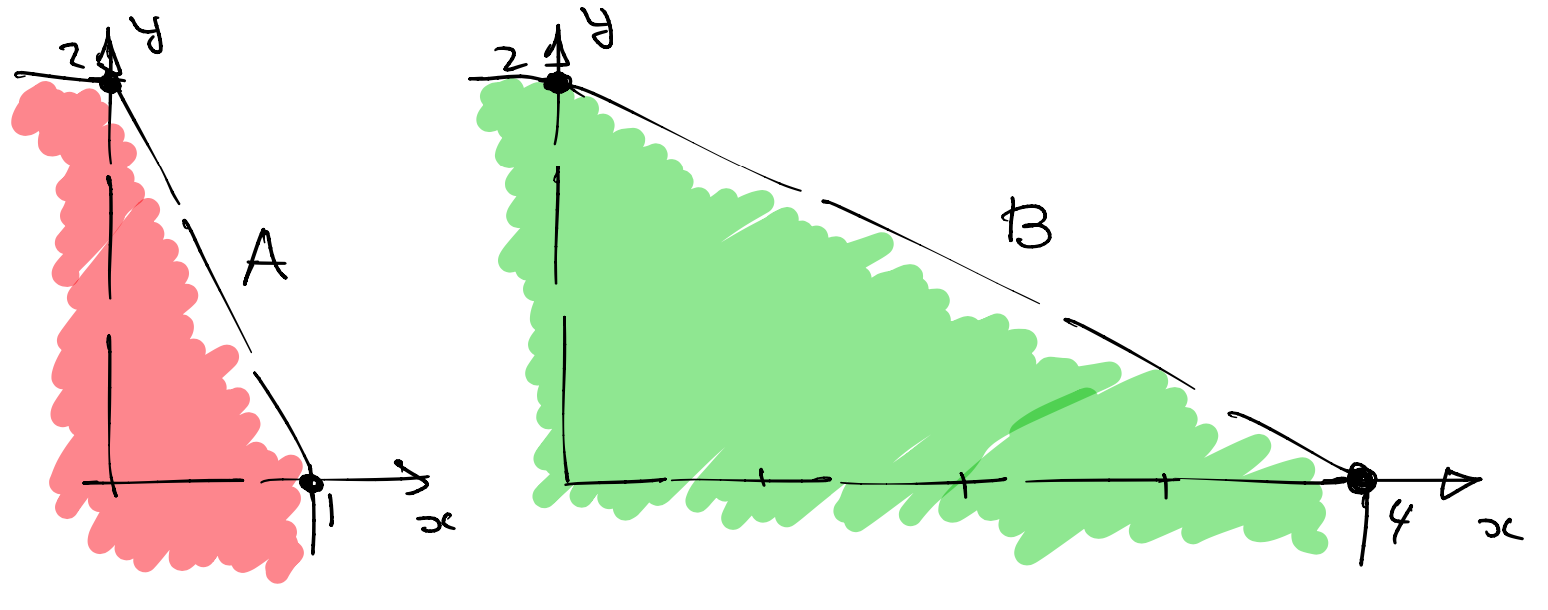
\includegraphics[width=1 \textwidth]{pic2.png}
\end{figure}
Пусть цена товара $x$ нормирована $p=1$, а товара $y$ равна $q$.
\end{frame}

\begin{frame}{Пример 2}
Найдем равновесие в автаркии для первой страны $A$. 

Опуская индекс страны, получаем УПП:
$$ \frac{U^{'}_x(x,y)}{U^{'}_y(x,y)} = \frac{1/x}{1/y} = \frac{1}{q} = \frac{1}{1/2} = \frac{F^{'}_X(X,Y)}{F^{'}_Y(X,Y)}$$
Моментально получаем что $q = 1/2$ и $y = 2x$.

Подставляя в соответствующие технологические границы, мы получаем координаты потребления $x = 1/2, y = 1$ и полезность $$U^{aut}_A = \log(1/2) + \log(1).$$

\end{frame}

\begin{frame}{Пример 2}
Найдем равновесие в автаркии для второй страны $B$. 

Опуская индекс страны, получаем УПП:
$$ \frac{U^{'}_x(x,y)}{U^{'}_y(x,y)} = \frac{1/x}{1/y} = \frac{1}{q} = \frac{1/4}{1/2} = \frac{F^{'}_X(X,Y)}{F^{'}_Y(X,Y)}$$
Моментально получаем что $q = 2$ и $y = x/2$.

Подставляя в соответствующие технологические границы, мы получаем координаты потребления $x = 2, y = 1$ и полезность $$U^{aut}_B = \log(2) + \log(1).$$

\end{frame}

\begin{frame}{Пример 2}
Найдем равновесие при международной торговле

Для этого надо понять, в каком из трех режимов работает экономика:

\begin{itemize}
  \item 1) $q = 1/2$, то есть страна $A$ не заметила разницы
  \item 2) $q = 2$, то есть страна $B$ не заметила разницы 
  \item 3) $q \in (1/2,2)$, то есть обе страны строго выиграли
\end{itemize}
Это легко визуализировать на совместной КПВ
\end{frame}

\begin{frame}{Пример 2}
\begin{figure}[hbt]
\centering
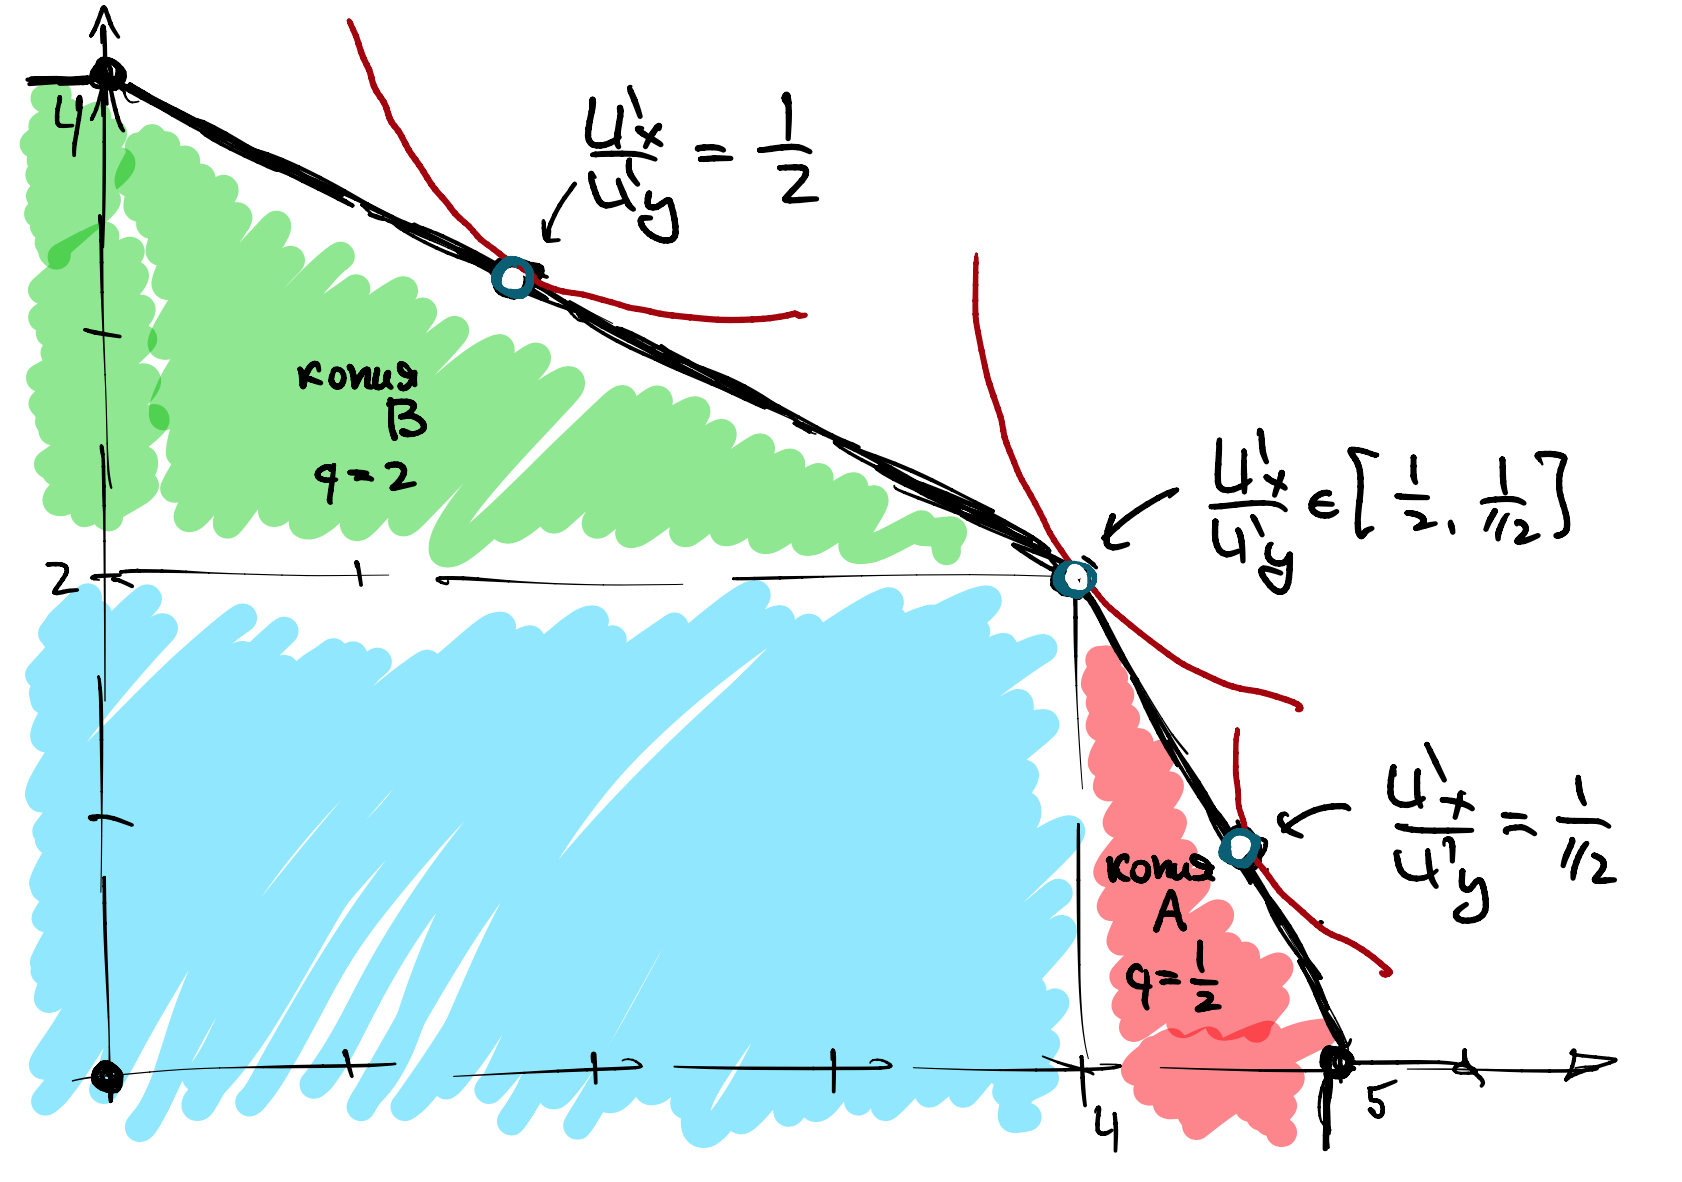
\includegraphics[width=1 \textwidth]{pic4.png}
\end{figure}
\end{frame}

\begin{frame}{Пример 2}
Далее будет перебор случаев, поэтому рекомендую завести табличку (даже несколько)

$$\begin{array}{c|c|c|c|c}
  \text{страна} & X & Y & x & y \\
  \hline
  A & & & &\\
  \hline
  B & & & &
\end{array}$$

\end{frame}

\section{Случай $q = 1/2$}

\begin{frame}{Пример 2}
Если $q = 1/2$ то мы находимся на <<правой арке>> КПВ
\begin{itemize}
  \item страна $A$ не заметила разницы между автаркией и международной торговлей, то есть $$x_A = 1/2, \ y_A = 1$$ но производить она может любую точку вдоль старой КПВ
  \item страна $B$ производит только первый товар, то есть
 $$X_B = 4, \ Y_B = 0$$
 но покупает какую-то внутреннюю точку
\end{itemize}
\end{frame}

\begin{frame}{Пример 2}
Мы разом заполнили половину таблички
$$\begin{array}{c|c|c|c|c}
  \text{страна} & X & Y & x & y \\
  \hline
  A & & & 1/2 & 1\\
  \hline
  B & 4 & 0 & &
\end{array}$$
\end{frame}

\begin{frame}{Пример 2}
Соответственно бюджет во второй стране равен $$4 p + 0 q = 4.$$ Спрос во второй стране выводится по формулам кобб-дугласа $$x_B = \frac{4}{2p} = 2, \ y_B = \frac{4}{2q} = 2/q = 4.$$
Мы заполнили табличку еще больше
$$\begin{array}{c|c|c|c|c}
  \text{страна} & X & Y & x & y \\
  \hline
  A & & & 1/2 & 1\\
  \hline
  B & 4 & 0 & 2 & 4
\end{array}$$
\end{frame}

\begin{frame}{Пример 2}
$$\begin{array}{c|c|c|c|c}
  \text{страна} & X & Y & x & y \\
  \hline
  A & & & 1/2 & 1\\
  \hline
  B & 4 & 0 & 2 & 4
\end{array}$$
Наконец, первой стране ничего не остается как произвести
\begin{align*}
	X_A & = x_A + x_B - X_B = 1/2 + 2 - 4 = -3/2\\
	Y_A & = y_A + y_B - Y_b = 1 + 4 - 0 = 5 
\end{align*}
Это явно противоречие, потому что \alert{в трейде, как правило, нельзя производить отрицательные количества товаров}, все товары потребительские. 

Однако, в домашке у вас будет специально по-другому. 
\end{frame}

\section{Случай $q = 2$}

\begin{frame}{Пример 2}
Если $q = 2$ то мы находимся на <<левой арке>> КПВ
\begin{itemize}
  \item страна $B$ не заметила разницы между автаркией и международной торговлей, то есть $$x_B = 2, \ y_B = 1$$
  \item страна $A$ производит только второй товар, то есть
 $$X_A = 0, \ Y_A = 2$$
 но покупает какую-то внутреннюю точку
\end{itemize}
\end{frame}

\begin{frame}{Пример 2}
Соответственно бюджет в первой стране равен $2q$. Спрос в первой стране выводится по формулам кобб-дугласа $$x_A = \frac{2q}{2p} = 2, \ y_A = \frac{2q}{2q} = 1 $$
Наконец, второй стране ничего не остается как произвести
\begin{align*}
	X_A & = x_a + x_b - X_B = 2 + 2 - 0 = 4\\
	Y_A & = y_a + y_b - Y_b = 1 + 1 - 2 = 0 
\end{align*}
Чудесным образом, это попадает в КПВ первой страны, УРА!!!
\end{frame}

\section{Случай $q \in (1/2,2)$}

\begin{frame}{Пример 2}
Если $q \in (1/2,2)$ то мы находимся на <<изломе>> КПВ
\begin{itemize}
  \item страна $A$ производит только второй товар, то есть
 $$X_A = 0, \ Y_A = 2$$
  \item страна $B$ производит только первый товар, то есть
 $$X_B = 4, \ Y_B = 0$$
\end{itemize}
При этом каждая страна покупает внутреннюю точку
\end{frame}

\begin{frame}{Пример 2}
Бюджет первой страны равен $2q$ а спрос соответственно
$$x_A = \frac{2q}{2p} = q, \quad y_A = \frac{2q}{2q} = 1 $$

Бюджет второй страны равен $4$ а спрос соответственно
$$x_B = \frac{4}{2p} = 2, \quad y_B = \frac{4}{2q} = 2/q $$

Приравнивая избыточный спрос $x$ к нулю получаем 
$$x_a + x_b - X_a - X_b = q + 2 - 0 - 4 = 0 \quad \Rightarrow \quad q = 2.$$

Формально, это противоречие, потому что $q \in (1/2,2)$.

\end{frame}

\section{Как перебирать случаи}

\begin{frame}{Пример 2}

Если вы не можете угадать режим решения с самого начала, рекомендую начать с <<излома>>, и если цена не попала в интервал перейти сразу к тому случаю, на который она пытается вам <<указать>>.

В данном случае, цена $q$ оказалась справа от интервала $(1/2,2)$ соответственно правильный режим это $q = 2$, или <<левая верхняя арка>> КПВ.

Но правильное решение тем не менее на изломе, так бывает если случайно сильно (не-)повезет с параметрами задачи.
\end{frame}

\section{Трейд, новый пример 3}

\begin{frame}{Пример 3}

Рассмотрим более сложный пример, с <<разными>> агентами.

Пусть у нас <<сферические>> технологии
$$ F^A(X,Y) = X^2 + Y^2 - 16 \leqslant 0, \quad F^B(X,Y) = X^2 + Y^2 - 9 \leqslant 0$$
Полезность Кобб Дуглас у первого: $$U^A(x,y) = \log x + \log y$$
и Леонтьев у второго $$U^B(x,y) = \min(x, \sqrt{2} y)$$
\end{frame}

\begin{frame}{Пример 3}
Найдем равновесие в автаркии для первой страны $A$. 

Опуская индекс страны, получаем УПП:
$$ \frac{U^{'}_x(x,y)}{U^{'}_y(x,y)} = \frac{1/x}{1/y} = \frac{p}{q} = \frac{2X}{2Y} = \frac{F^{'}_X(X,Y)}{F^{'}_Y(X,Y)}$$
Моментально получаем что $x = y$ и $p = q$.

Подставляя в соответствующие технологические границы, мы получаем координаты потребления $x = 4, y = 4$ и полезность $$U^{aut}_A = 2 \log 4.$$

\end{frame}

\begin{frame}{Пример 3}
Найдем равновесие в автаркии для второй страны $B$. 

Помним, что интересующее нас геометрическое место точек описывается уравнением
$$x = \sqrt{2} y$$

Подставляя в соответствующие технологические границы, мы получаем координаты потребления $x = \sqrt{6}, y = \sqrt{3}$ и $$U^{aut}_B = \sqrt{6}$$
Цены можно, по прежнему, вытащить из фоков для фирмы
$$ \frac{p}{q} = \frac{2X}{2Y} = \frac{F^{'}_X(X,Y)}{F^{'}_Y(X,Y)}.$$
\end{frame}

\begin{frame}{Пример 3}
Попробуем общее равновесие.

Для построения совместного КПВ можно
\begin{itemize}
  \item воспользоваться геометрической интуицией
  \item построить руками через наклон
  \item max $X_{sum}$ при заданном $Y_{sum}$ или наоборот.
\end{itemize}
Последний подход мне сейчас нравится больше всего.
\end{frame}

\begin{frame}{Пример 3}
Но в этой задаче нам это даже и не поможет, поэтому придется идти через избыточный спрос...

Пусть цены нормированы к $(1,q)$.
$$\begin{array}{c|c|c|c|c}
  \text{страна} & X & Y & x & y \\
  \hline
  A & ? & ? & ? &\\
  \hline
  B & ? & ? & ? &
\end{array}$$
Чтобы найти $q$ достаточно узнать все про товар $x$:
$$ x_A(q) + x_B(q) - X_A(q) - X_B(q) = 0$$
...немного подумав, убеждаемся что \alert{вычитать запасы тут не надо, потому что это трейд, тут запасы зашиты в $X,Y$}. Да и как их вычесть, если они в задаче даже не известны?
\end{frame}

\end{document}
